% =====================================================================
%   Conversational EDA Chatbot & E-Commerce Churn Prediction - POSTER
%   Authors:   Tuyiramye Christian (2517025)
%              Dushime Pacifique  (2517004)
%   Supervisor: Prof. Dr. Jebran Khan
%   Department: Artificial Intelligence  |  Spring 2025
%
%   Compile with:
%     pdflatex poster.tex
%     pdflatex poster.tex
%
%   Output: A0 portrait poster (841 mm x 1189 mm)
% =====================================================================
\documentclass[25pt, a0paper, portrait,
               margin=0mm, innermargin=14mm,
               blockverticalspace=10mm, colspace=14mm,
               subcolspace=8mm]{tikzposter}

% ---------- Packages ----------
\usepackage[utf8]{inputenc}
\usepackage[T1]{fontenc}
\usepackage{lmodern}
\usepackage{amsmath,amssymb}
\usepackage{graphicx}
\usepackage{booktabs}
\usepackage{tabularx}
\usepackage{array}
\usepackage{xcolor}
\usepackage{enumitem}
\setlist{leftmargin=14pt, itemsep=2pt, topsep=2pt}

\usepackage{tikz}
\usetikzlibrary{
  arrows.meta, positioning, shapes.geometric,
  fit, backgrounds, calc
}
\usepackage{pgfplots}
\pgfplotsset{compat=1.18}

% ---------- Disable tikzposter's promo footer ----------
\tikzposterlatexaffectionproofoff

% ---------- Theme + colors ----------
\usetheme{Default}
\usecolorstyle{Britain}      % deep blue palette
\useblockstyle{Default}
\usetitlestyle{Filled}

% ---------- Project palette (matches theme) ----------
\definecolor{pBlue}{HTML}{1E3C72}
\definecolor{pBlueLight}{HTML}{2A5298}
\definecolor{pOrange}{HTML}{E76F51}
\definecolor{pTeal}{HTML}{2A9D8F}
\definecolor{pYellow}{HTML}{F4A261}
\definecolor{pGray}{HTML}{4B5563}

% ---------- Title block ----------
\title{\parbox{\linewidth}{\centering
       Conversational EDA Chatbot \\[6pt]
       \textit{\&} \\[6pt]
       E-Commerce Customer Churn Prediction}}
\author{Tuyiramye Christian \,(ID: 2517025) \quad\textbullet\quad
        Dushime Pacifique \,(ID: 2517004)}
\institute{Supervisor: \textbf{Prof.\ Dr.\ Jebran Khan} \\[4pt]
           Department of Artificial Intelligence \,\textbullet\, Spring 2025}

% =====================================================================
\begin{document}
% =====================================================================
\maketitle

% ============================ ROW 1 ==================================
\begin{columns}

% ---------- COLUMN 1 ----------
\column{0.34}

\block{1.\, Motivation}{
\textbf{Two pain points} plague modern e-commerce analytics:
\begin{itemize}
  \item \textbf{Data-access bottleneck.} Stakeholders wait hours or
        days for analysts to write SQL, killing iterative exploration.
  \item \textbf{Reactive retention.} Churn is discovered \emph{after}
        revenue loss; acquiring a new customer costs \textbf{5--25$\times$}
        more than retaining one.
\end{itemize}
\vspace{4pt}
\textbf{Our solution} is a unified analytics platform with two
artifacts that share the same data domain:
\begin{enumerate}
  \item A \textbf{conversational EDA chatbot} that turns natural
        language into safe SQL and interactive charts.
  \item A \textbf{churn-prediction pipeline} that ranks at-risk
        customers so retention spending is targeted.
\end{enumerate}
}

\block{2.\, Objectives}{
\begin{itemize}
  \item Translate plain English $\to$ syntactically valid MySQL.
  \item Dynamic output: \textbf{table}, \textbf{summary}, or
        \textbf{interactive chart}.
  \item Strict \textbf{read-only} guardrails.
  \item Multi-turn \textbf{conversational memory}.
  \item Train and evaluate a churn classifier with leakage-free
        cross-validation, hyperparameter tuning, and interpretability.
  \item Ship \textbf{portable, modular} artifacts (one .py + one .ipynb).
\end{itemize}
}

\block{3.\, Technology Stack}{
\begin{center}
\small
\begin{tabular}{@{}ll@{}}
\toprule
\textbf{Layer} & \textbf{Technology} \\
\midrule
Chat UI            & Streamlit \\
LLM orchestration  & LangChain (+Experimental) \\
Language model     & OpenAI GPT-4o, $T=0$ \\
Database           & MySQL via \texttt{pymysql} \\
Visualization      & Plotly Express, Matplotlib \\
ML Modeling        & scikit-learn \\
Notebook           & Jupyter \\
Runtime            & Python 3.11 \\
\bottomrule
\end{tabular}
\end{center}
}

% ---------- COLUMN 2 ----------
\column{0.33}

\block{4.\, System Architecture}{
\begin{center}
\begin{tikzpicture}[
  node distance=0.7cm and 1.0cm,
  every node/.style={font=\small},
  user/.style={ellipse, draw=pBlue, fill=pBlue!12, line width=1pt,
               minimum width=4.6cm, minimum height=1.1cm, align=center},
  ui/.style={rectangle, draw=pBlueLight, fill=pBlueLight!12, line width=1pt,
             rounded corners=4pt, minimum width=5.4cm, minimum height=1.2cm, align=center},
  agent/.style={rectangle, draw=pOrange, fill=pOrange!12, line width=1pt,
                rounded corners=4pt, minimum width=5.8cm, minimum height=1.5cm, align=center},
  router/.style={diamond, aspect=2, draw=pYellow!70!black, fill=pYellow!25, line width=1pt,
                 minimum width=5.0cm, minimum height=0.8cm, align=center},
  out/.style={rectangle, draw=pTeal, fill=pTeal!15, line width=1pt,
              rounded corners=4pt, minimum width=4.8cm, minimum height=1.1cm, align=center},
  ar/.style={-{Latex[length=4mm]}, line width=1pt, draw=pGray}
]
  \node[user]                       (u)     {\textbf{Stakeholder}\\\small natural language};
  \node[ui, below=of u]             (ui)    {\textbf{Streamlit UI} (\texttt{app.py})};
  \node[agent, below=of ui]         (sql)   {\textbf{Phase A: SQL Agent}\\ \small ZSR-D\,/\,read-only prefix};
  \node[router, below=of sql]       (rt)    {\textbf{Visual router}};
  \node[out, below left=1.2cm and -0.3cm of rt] (tx) {Text / Table};
  \node[agent, below right=1.2cm and -0.3cm of rt] (pd) {\textbf{Phase B: Pandas Agent}\\ \small Plotly\,/\,Matplotlib code};
  \node[out, below=of pd]           (ch)    {\textbf{Sandboxed \texttt{exec()}} chart};
  \draw[ar] (u)--(ui); \draw[ar] (ui)--(sql); \draw[ar] (sql)--(rt);
  \draw[ar] (rt)--(tx); \draw[ar] (rt)--(pd); \draw[ar] (pd)--(ch);
\end{tikzpicture}
\end{center}
\vspace{4pt}
\textbf{Dual-agent design.} Phase~A generates SQL; Phase~B generates
visualization code only when the prompt contains a visual trigger.
}

\block{5.\, Phase A --- SQL Agent}{
\begin{itemize}
  \item Built with \texttt{create\_sql\_agent} using the
        \textbf{ZERO\_SHOT\_REACT\_DESCRIPTION} agent type.
  \item Executes a \emph{Thought $\to$ Action $\to$ Observation} loop
        over the \texttt{SQLDatabaseToolkit} (list tables, inspect
        schema, run query, check query).
  \item \textbf{Read-only system prefix} explicitly forbids
        \texttt{INSERT, UPDATE, DELETE, DROP, TRUNCATE, ALTER, CREATE,
        REPLACE, GRANT, REVOKE, RENAME, LOCK, CALL, MERGE}.
  \item Hardened: \texttt{handle\_parsing\_errors=True},
        \texttt{max\_iterations=12},
        \texttt{sample\_rows\_in\_table\_info=3}.
  \item Connection pooled via \texttt{@st.cache\_resource}.
\end{itemize}
}

\block{6.\, Phase B --- Visualization Sandbox}{
\begin{center}
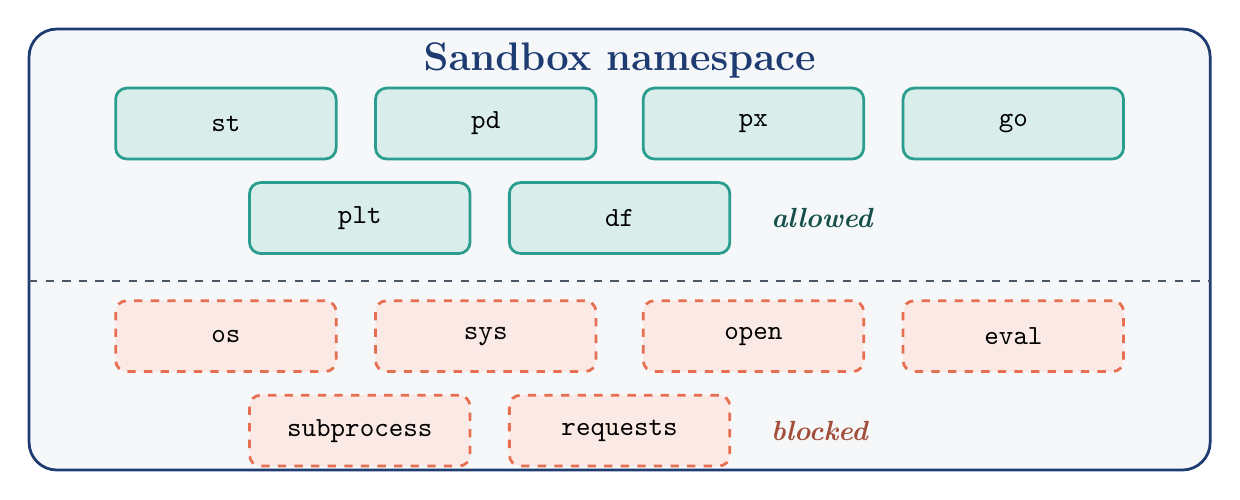
\begin{tikzpicture}[
  every node/.style={font=\normalsize},
  ok/.style={rectangle, rounded corners=4pt, draw=pTeal, fill=pTeal!18,
             minimum width=2.8cm, minimum height=0.9cm, align=center, line width=1pt},
  bad/.style={rectangle, rounded corners=4pt, draw=pOrange, fill=pOrange!15, dashed,
              minimum width=2.8cm, minimum height=0.9cm, align=center, line width=1pt}
]
\draw[draw=pBlue, line width=1pt, rounded corners=10pt, fill=pBlue!4]
  (-7.5,-2.6) rectangle (7.5,3.0);
\node[anchor=north, font=\Large\bfseries, color=pBlue]
  at (0,2.95) {Sandbox namespace};

\node[ok] at (-5.0, 1.8)  {\texttt{st}};
\node[ok] at (-1.7, 1.8)  {\texttt{pd}};
\node[ok] at ( 1.7, 1.8)  {\texttt{px}};
\node[ok] at ( 5.0, 1.8)  {\texttt{go}};
\node[ok] at (-3.3, 0.6)  {\texttt{plt}};
\node[ok] at ( 0.0, 0.6)  {\texttt{df}};
\node[anchor=west, font=\itshape, color=pTeal!50!black] at (1.8,0.6) {\textbf{allowed}};

\draw[dashed, draw=pGray] (-7.5,-0.2) -- (7.5,-0.2);

\node[bad] at (-5.0,-0.9) {\texttt{os}};
\node[bad] at (-1.7,-0.9) {\texttt{sys}};
\node[bad] at ( 1.7,-0.9) {\texttt{open}};
\node[bad] at ( 5.0,-0.9) {\texttt{eval}};
\node[bad] at (-3.3,-2.1) {\texttt{subprocess}};
\node[bad] at ( 0.0,-2.1) {\texttt{requests}};
\node[anchor=west, font=\itshape, color=pOrange!70!black] at (1.8,-2.1) {\textbf{blocked}};
\end{tikzpicture}
\end{center}
\vspace{4pt}
\textbf{Three-layer defense.} (1)~prompt-level restriction,
(2)~namespace-level restriction (only six names in scope),
(3)~broad \texttt{try/except} so the Streamlit thread never crashes.
}

% ---------- COLUMN 3 ----------
\column{0.33}

\block{7.\, ML Pipeline}{
\begin{center}
\begin{tikzpicture}[
  node distance=0.4cm and 0.3cm,
  every node/.style={font=\small},
  step/.style={rectangle, rounded corners=4pt, line width=1pt,
               draw=pBlue, fill=pBlue!10,
               minimum width=3.0cm, minimum height=1.4cm, align=center},
  ar/.style={-{Latex[length=3mm]}, line width=1pt, draw=pGray}
]
\node[step] (a) {Synthetic\\ Dataset\\ \scriptsize 5{,}000};
\node[step, right=of a] (b) {Pre-\\process\\ \scriptsize scale+OHE};
\node[step, right=of b] (c) {Train/\\Test\\ \scriptsize 80/20};
\node[step, right=of c] (d) {5-fold\\ CV\\ \scriptsize LR/RF/GBM};
\node[step, right=of d] (e) {Grid\\ Search\\ \scriptsize tune};
\node[step, right=of e] (f) {Evaluate\\ \scriptsize ROC/PR/CM};
\foreach \i/\j in {a/b,b/c,c/d,d/e,e/f} \draw[ar] (\i)--(\j);
\end{tikzpicture}
\end{center}
\textbf{Reproducible} 5{,}000-customer e-commerce dataset
generated with \texttt{seed=42}. Eleven features span demographics
(age, gender, region), account (tier, payment, tenure), and behavior
(AOV, cadence, return rate, support tickets, recency, discount usage).
}

\block{8.\, Results}{
\begin{center}
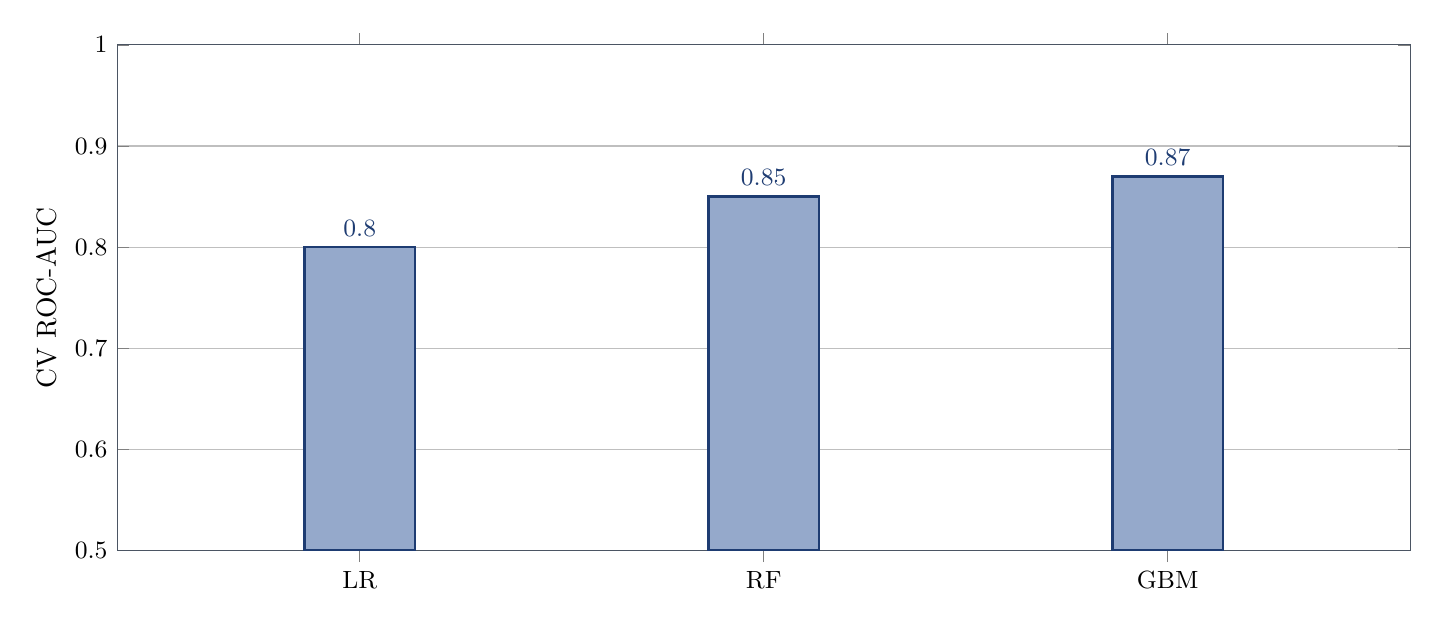
\begin{tikzpicture}
\begin{axis}[
  width=18cm, height=8cm,
  ybar, bar width=40pt,
  ymin=0.5, ymax=1.0, ymajorgrids,
  ylabel={CV ROC-AUC},
  symbolic x coords={LR, RF, GBM},
  xtick=data,
  nodes near coords,
  every node near coord/.append style={font=\small, color=pBlue},
  tick label style={font=\small},
  enlarge x limits=0.3,
  axis line style={draw=pGray}
]
\addplot+[draw=pBlue, fill=pBlueLight!50, line width=1pt]
  coordinates {(LR,0.80) (RF,0.85) (GBM,0.87)};
\end{axis}
\end{tikzpicture}
\end{center}
\vspace{4pt}

\begin{center}
\small
\begin{tabular}{@{}lcc@{}}
\toprule
\textbf{Model} & \textbf{CV ROC-AUC} & \textbf{Std} \\
\midrule
Gradient Boosting    & \textbf{0.87} & 0.010 \\
Random Forest        & 0.85 & 0.011 \\
Logistic Regression  & 0.80 & 0.012 \\
\bottomrule
\end{tabular}
\end{center}
\textbf{Tuned Gradient Boosting} wins; ensembles beat the linear
baseline by a clear margin on the held-out test set.
}

\block{9.\, Top Churn Drivers}{
\begin{center}
\begin{tikzpicture}
\begin{axis}[
  width=18cm, height=12cm,
  xbar, bar width=14pt,
  xmin=0, xmax=0.18,
  xlabel={Permutation $\Delta$ROC-AUC},
  symbolic y coords={
    discount, age, gender, region, payment,
    orders/mo, tenure, tickets,
    tier=Gold, tier=Platinum, return\_rate, recency
  },
  ytick=data,
  tick label style={font=\small},
  nodes near coords,
  every node near coord/.append style={font=\small, color=pBlue},
  axis line style={draw=pGray}
]
\addplot+[draw=pBlue, fill=pBlueLight!50, line width=1pt]
  coordinates {
    (0.005, discount)
    (0.007, age)
    (0.008, gender)
    (0.010, region)
    (0.012, payment)
    (0.020, orders/mo)
    (0.025, tenure)
    (0.040, tickets)
    (0.055, tier=Gold)
    (0.065, tier=Platinum)
    (0.110, return\_rate)
    (0.155, recency)
  };
\end{axis}
\end{tikzpicture}
\end{center}
\textbf{Recency} and \textbf{return rate} dominate;
\textbf{loyalty tiers} (Gold, Platinum) protect against churn.
}

\end{columns}

% ============================ ROW 2 ==================================
\begin{columns}
\column{0.5}
\block{10.\, Conclusion}{
We deliver a coherent two-part analytics solution:
a \textbf{secure conversational EDA chatbot} that turns plain English
into SQL queries and interactive charts, and a \textbf{rigorous
churn-prediction pipeline} that ranks customers by retention risk.
Both components ship with production discipline: caching, error
handling, security guardrails, reproducibility, and clean modular
code. Together they cover the \textbf{descriptive} and
\textbf{predictive} halves of customer analytics in one platform.
}

\column{0.5}
\block{11.\, Future Work \& Acknowledgments}{
\textbf{Future work.}
\begin{itemize}
  \item Replace the keyword router with an LLM-as-judge intent
        classifier.
  \item Retrain on the live MySQL warehouse via the same connection.
  \item Per-customer SHAP attributions for personalized retention
        offers.
  \item Cost-sensitive threshold tuning + LangSmith observability.
\end{itemize}
\vspace{4pt}
\textbf{Acknowledgments.} We sincerely thank our supervisor
\textbf{Prof.\ Dr.\ Jebran Khan} for his expert guidance and
constructive feedback throughout this project, and the
\textbf{Department of Artificial Intelligence} for its support.
}
\end{columns}

% ============================ ROW 3: Footer ==========================
\block{}{
\begin{center}
\small
\textbf{Tuyiramye Christian} (2517025) \quad\textbullet\quad
\textbf{Dushime Pacifique} (2517004) \quad\textbullet\quad
Supervisor: \textbf{Prof.\ Dr.\ Jebran Khan} \quad\textbullet\quad
Department of Artificial Intelligence \quad\textbullet\quad
\textbf{Spring 2025}
\end{center}
}

\end{document}
